%% BioMed_Central_Tex_Template_v1.06
%%                                      %
%  bmc_article.tex            ver: 1.06 %
%                                       %

%%IMPORTANT: do not delete the first line of this template

%%%%%%%%%%%%%%%%%%%%%%%%%%%%%%%%%%%%%%%%%
%%                                     %%
%%  LaTeX template for BioVis 2014  %%
%%      article submissions     %%
%%          adapted from BMC    %%
%%          <8 Jan 2014>              %%
%% Liz Marai (g.elisabeta.marai@gmail.com) %%
%%                                     %%
%%%%%%%%%%%%%%%%%%%%%%%%%%%%%%%%%%%%%%%%%


%%%%%%%%%%%%%%%%%%%%%%%%%%%%%%%%%%%%%%%%%%%%%%%%%%%%%%%%%%%%%%%%%%%%%
%%                                                                 %%
%%%%%%%%%%%%%%%%%%%%%%%%%%%%%%%%%%%%%%%%%%%%%%%%%%%%%%%%%%%%%%%%%%%%%

%%% additional documentclass options:
%  [doublespacing]
%  [linenumbers]   - put the line numbers on margins

%%% loading packages, author definitions

\documentclass[twocolumn]{bmcart}% uncomment this for twocolumn layout 



%%% Load packages
%\usepackage{amsthm,amsmath}
%\RequirePackage{natbib}
%\RequirePackage{hyperref}
\usepackage[utf8]{inputenc} %unicode support
%\usepackage[applemac]{inputenc} %applemac support if unicode package fails
%\usepackage[latin1]{inputenc} %UNIX support if unicode package fails
\usepackage{graphicx}

%%%%%%%%%%%%%%%%%%%%%%%%%%%%%%%%%%%%%%%%%%%%%%%%%
%%                                             %%
%%  If you wish to display your graphics for   %%
%%  your own use using includegraphic or       %%
%%  includegraphics, then comment out the      %%
%%  following two lines of code.               %%
%%%%%%%%%%%%%%%%%%%%%%%%%%%%%%%%%%%%%%%%%%%%%%%%%


%\def\includegraphic{}
%\def\includegraphics{}



%%% Put your definitions there:
\startlocaldefs
\endlocaldefs


%%% Begin ...
\begin{document}

%%% Start of article front matter
\begin{frontmatter}

\begin{fmbox}
\dochead{Research}

%%%%%%%%%%%%%%%%%%%%%%%%%%%%%%%%%%%%%%%%%%%%%%
%%                                          %%
%% Enter the title of your article here     %%
%%                                          %%
%%%%%%%%%%%%%%%%%%%%%%%%%%%%%%%%%%%%%%%%%%%%%%

\title{Comparative Visualization of Molecular Secondary Structures}

%%%%%%%%%%%%%%%%%%%%%%%%%%%%%%%%%%%%%%%%%%%%%%
%%                                          %%
%% Do not enter the authors here for        %%
%%  a double-blind review. Otherwise        %%
%% specify information, if available,       %%
%% in the form:                             %%
%%   <key>={<id1>,<id2>}                    %%
%%   <key>=                                 %%
%% Comment or delete the keys which are     %%
%% not used. Repeat \author command as much %%
%% as required.                             %%
%%                                          %%
%%%%%%%%%%%%%%%%%%%%%%%%%%%%%%%%%%%%%%%%%%%%%%
\author[
     addressref={aff1},
  % noteref={n2},
   email={lucia.koc@gmail.com}
]{\inits{LK}\fnm{Lucia} \snm{Kocincov\'{a}}}
\author[
   addressref={aff1},                   % id's of addresses, e.g. {aff1,aff2}
   %corref={aff1},                       % id of corresponding address, if any
   %noteref={n1},                        % id's of article notes, if any
  email={jaresova@mail.muni.cz}   % email address
]{\inits{MJ}\fnm{Miroslava} \snm{Jare\v{s}ov\'{a}}}
\author[
   addressref={aff1,aff2},                   % id's of addresses, e.g. {aff1,aff2}
   %corref={aff1},                       % id of corresponding address, if any
   %noteref={n1},                        % id's of article notes, if any
  email={xbyska@fi.muni.cz}   % email address
]{\inits{JB}\fnm{Jan} \snm{By\v{s}ka}}
\author[
   addressref={aff2},                   % id's of addresses, e.g. {aff1,aff2}
   %corref={aff1},                       % id of corresponding address, if any
   %noteref={n1},                        % id's of article notes, if any
  email={julius.parulek@uib.no}   % email address
]{\inits{JP}\fnm{J\'{u}lius} \snm{Parulek}}
\author[
   addressref={aff2},                   % id's of addresses, e.g. {aff1,aff2}
   %corref={aff1},                       % id of corresponding address, if any
   %noteref={n1},                        % id's of article notes, if any
  email={Helwig.Hauser@uib.no}   % email address
]{\inits{HH}\fnm{Helwig} \snm{Hauser}}
\author[
   addressref={aff1},                   % id's of addresses, e.g. {aff1,aff2}
   %corref={aff1},                       % id of corresponding address, if any
   %noteref={n1},                        % id's of article notes, if any
  email={kozlikova@fi.muni.cz}   % email address
]{\inits{BK}\fnm{Barbora} \snm{Kozl\'{i}kov\'{a}}}


%%%%%%%%%%%%%%%%%%%%%%%%%%%%%%%%%%%%%%%%%%%%%%
%%                                          %%
%% Enter the authors' addresses here        %%
%%                                          %%
%% Repeat \address commands as much as      %%
%% required.                                %%
%%                                          %%
%%%%%%%%%%%%%%%%%%%%%%%%%%%%%%%%%%%%%%%%%%%%%%

\address[id=aff1]{%                           % unique id
  \orgname{Masaryk University}, % university, etc
 % \postcode{60200}                                % post or zip code
  \city{Brno},                              % city
  \cny{Czech Republic}                                    % country
}
\address[id=aff2]{%                           % unique id
  \orgname{University of Bergen}, % university, etc
%  \street{210 South Bouquet},                     %
  %\postcode{15260}                                % post or zip code
  %\city{Bergen},                              % city
  \cny{Norway}                                    % country
}


%%%%%%%%%%%%%%%%%%%%%%%%%%%%%%%%%%%%%%%%%%%%%%
%%                                          %%
%% Enter short notes here                   %%
%%                                          %%
%% Short notes will be after addresses      %%
%% on first page.                           %%
%%                                          %%
%%%%%%%%%%%%%%%%%%%%%%%%%%%%%%%%%%%%%%%%%%%%%%

\begin{artnotes}
%\note{Sample of title note}     % note to the article
%\note[id=n1]{Equal contributor} % note, connected to author
%\note[id=n2]{Equal contributor} % note, connected to author
%\note[id=n3]{Equal contributor} % note, connected to author
%\note[id=n4]{Project leader and equal contributor} % note, connected to author
\end{artnotes}

\end{fmbox}% comment this for two column layout

%%%%%%%%%%%%%%%%%%%%%%%%%%%%%%%%%%%%%%%%%%%%%%
%%                                          %%
%% The Abstract begins here                 %%
%%                                          %%
%% Please refer to the Instructions for     %%
%% authors on http://www.biomedcentral.com  %%
%% and include the section headings         %%
%% accordingly for your article type.       %%
%%                                          %%
%%%%%%%%%%%%%%%%%%%%%%%%%%%%%%%%%%%%%%%%%%%%%%

\begin{abstractbox}

\begin{abstract} % abstract, must be under 350 words
%\parttitle{First part title} %if any
%Text for this section.
  

\parttitle{Background} Visual comparison of molecular structures could provide domain experts with an important information about the similarities and differences in their protein chains. Information about the amino acids (AA) is typically conveyed via secondary structures or as a 1D sequence of AA forming the protein chain. 

\parttitle{Results} We propose a new visualization technique that bridges these two commonly used representations and by which we are able to compare multiple proteins. Our technique improves the 1D sequential representation by adding parameters derived from geometry of secondary structures, which includes their length and spatial orientation. Further, we introduce a  way to utilize these geometrical aspects to compare two or more protein structures efficiently. The core of our technique is based on unrolling the protein chain to a line while maintaining the mutual orientation of secondary structures as well as their lengths. Then the user can explore in detail structures of interest, which are visually compared via superimposition and juxtaposition techniques. 

\parttitle{Conclusions}  We demonstrate the usability of our method on several representatives of the family of cytochromes P450 where the position of the secondary structures has a significant impact on the substrate channeling.

%\parttitle{Second part title} %if any
%Text for this section.
\end{abstract}

%%%%%%%%%%%%%%%%%%%%%%%%%%%%%%%%%%%%%%%%%%%%%%
%%                                          %%
%% The keywords begin here                  %%
%%                                          %%
%% Put each keyword in separate \kwd{}.     %%
%%                                          %%
%%%%%%%%%%%%%%%%%%%%%%%%%%%%%%%%%%%%%%%%%%%%%%

\begin{keyword}
\kwd{Molecular Sequence Analysis}
\kwd{Molecular Structural Biology}
\kwd{Computational Proteomics}
\end{keyword}

% MSC classifications codes, if any
%\begin{keyword}[class=AMS]
%\kwd[Primary ]{}
%\kwd{}
%\kwd[; secondary ]{}
%\end{keyword}

\end{abstractbox}
%
%\end{fmbox}% uncomment this for twcolumn layout

\end{frontmatter}

%%%%%%%%%%%%%%%%%%%%%%%%%%%%%%%%%%%%%%%%%%%%%%
%%                                          %%
%% The Main Body begins here                %%
%%                                          %%
%% Please refer to the instructions for     %%
%% authors on:                              %%
%% http://www.biomedcentral.com/info/authors%%
%% and include the section headings         %%
%% accordingly for your article type.       %%
%%                                          %%
%% See the Results and Discussion section   %%
%% for details on how to create sub-sections%%
%%                                          %%
%% use \cite{...} to cite references        %%
%%  \cite{koon} and                         %%
%%  \cite{oreg,khar,zvai,xjon,schn,pond}    %%
%%  \nocite{smith,marg,hunn,advi,koha,mouse}%%
%%                                          %%
%%%%%%%%%%%%%%%%%%%%%%%%%%%%%%%%%%%%%%%%%%%%%%

%%%%%%%%%%%%%%%%%%%%%%%%% start of article main body
% <put your article body there>

%%%%%%%%%%%%%%%%
%% Background %%
%%
\section*{Background}

Our method aims to cover the gap between two commonly used representations of molecular structure. Moreover, the proposed solution serves for the comparison of multiple protein structures.
We focus on structure alignment which finds the best fitting of protein chains and align them with respect to the root mean square deviation (we are using the Combinatorial Extensions algorithm).
When studying the similarity between more proteins or the differences in whole protein families, the 3D representation is inapplicable because of the visual clutter caused by many intersections (image). This is very true even for small sets of proteins to compare (for very similar structures 5 and more, for structures with lot of differences 3 and more). Thus, in these cases the traditional sequential 1D information is used (image). Here the individual amino acids are aligned (TODO describe structure and sequence alignment and their difference?) and when each row of the representation represents one protein structure, the user can observe the similarities by studying the columns. Some methods allow to integrate the information about the secondary structures in these chains. However, the information about the spatial orientation of the corresponding secondary structures is completely lost. 
In our representation we utilize the fact that the users are trained to understand the sequential representation well but we add another crucial information about the mutual position of corresponding secondary structures. So our representation helps to reveal not only the differences in the sequence and length of corresponding secondary structures but also the differences in the spatial orientation of the corresponding SS. This is impossible to reach using the traditionally used 1D representation and reaching it in 3D representation is very complex task for large datasets because the user has to study the mutual alignment of proteins from this dataset in smaller portions and merge the gained information manually. 
Strong points of our representation:
\begin{itemize}
\item the domain experts are accustomed with the sequential representation as well as with secondary structures
\item interactive manipulation
\item predefined ranking according to RMSD
\item changing superimposition and juxtaposition
\item linking with 3D
\item automatic highlighting of the most similar and the most different secondary structures
\item filtering (removing the most different proteins)
\item coloring of SS in the abstracted representation with respect to the physico-chemical properties of the amino acids
\end{itemize}

Related work: \cite{Stolte2015}, maybe also \cite{Nguyen2013}

\section*{Methodology}
TODO 

\subsection*{Design}
\begin{figure*}[t!]
  \centering
  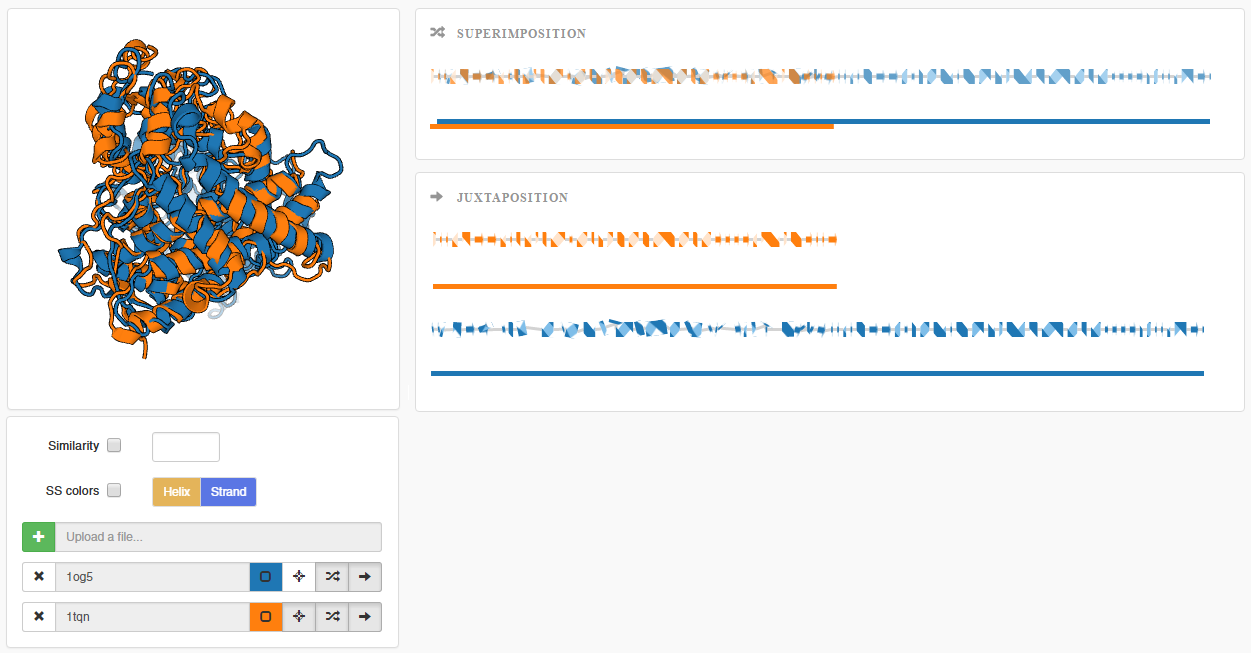
\includegraphics[height=3.5in]{pics/design.png}
  \caption{Overview of the system consisting of three main parts.}
  \label{fig:design}
\end{figure*}

\subsection*{Implementation}
With the use of the Combinatorial Extension (CE) algorithm for structure alignment~\cite{Shindyalov1998} and force layout algorithm, we let the structures to align in 3D, so there is no deformation caused by choosing a particular projection or distortion. 
At the end, we visualize the flattened molecules as if they were stretched out from 3D by pulling the chosen reference molecule at its ends into a straight line, so the actual length of secondary structures is preserved as well as the position of near structures of other molecules which are “locked” to the reference molecule.

Algorithm

\subsection*{Interaction}


%\begin{figure*}[t!]
%  \centering
%  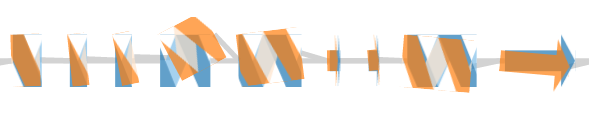
\includegraphics[height=3.5in]{pics/teaser.png}
%  \caption{Example two-column figure. To insert a single column figure, remove the * in the two figure tags. }
%  \label{fig:interface}
%\end{figure*}


\section*{Results and Discussion}
TODO

\subsection*{Case Study}

\section*{Conclusions}
TODO

Future work
%%%%%%%%%%%%%%%%%%%%%%%%%%%%%%%%%%%%%%%%%%%%%% 
%%                                          %%
%% Backmatter begins here                   %%
%%                                          %%
%%%%%%%%%%%%%%%%%%%%%%%%%%%%%%%%%%%%%%%%%%%%%%

\begin{backmatter}

%\section*{List of abbreviations used}
%TIM: \textit{triosephosphate isomerase}, scTIM: \textit{saccharomyces
%cerevisiae triosephosphate isomerase}, dTIM: \textit{defective triosephosphate
%isomerase}, PDB: \textit{protein data bank}.

\section*{Competing interests}
The authors declare that they have no competing interests.


%%%%%%%%%%%%%%%%%%%%%%%%%%%%%%%%%%%%%%%%%%%%%%%%%%%%%%%%%%%%%
%%                  The Bibliography                       %%
%%                                                         %%
%%  Bmc_mathpys.bst  will be used to                       %%
%%  create a .BBL file for submission.                     %%
%%  After submission of the .TEX file,                     %%
%%  you will be prompted to submit your .BBL file.         %%
%%                                                         %%
%%                                                         %%
%%  Note that the displayed Bibliography will not          %%
%%  necessarily be rendered by Latex exactly as specified  %%
%%  in the online Instructions for Authors.                %%
%%                                                         %%
%%%%%%%%%%%%%%%%%%%%%%%%%%%%%%%%%%%%%%%%%%%%%%%%%%%%%%%%%%%%%

% if your bibliography is in bibtex format, use those commands:
\bibliographystyle{bmc-mathphys} % Style BST file
\bibliography{bmc_article}      % Bibliography file (usually '*.bib' )

% or include bibliography directly:
% \begin{thebibliography}
% \bibitem{b1}
% \end{thebibliography}

%%%%%%%%%%%%%%%%%%%%%%%%%%%%%%%%%%%
%%                               %%
%% Figures                       %%
%%                               %%
%% NB: this is for captions and  %%
%% Titles. All graphics must be  %%
%% submitted separately and NOT  %%
%% included in the Tex document  %%
%%                               %%
%%%%%%%%%%%%%%%%%%%%%%%%%%%%%%%%%%%

%%
%% Do not use \listoffigures as most will included as separate files

%\section*{Figures}
%  \begin{figure}[h!]
 % \caption{\csentence{Sample figure title.}
  %    A short description of the figure content
   %   should go here.}
   %   \end{figure}

%\begin{figure}[h!]
 % \caption{\csentence{Sample figure title.}
  %    Figure legend text.}
  %    \end{figure}

%%%%%%%%%%%%%%%%%%%%%%%%%%%%%%%%%%%
%%                               %%
%% Tables                        %%
%%                               %%
%%%%%%%%%%%%%%%%%%%%%%%%%%%%%%%%%%%

%% Use of \listoftables is discouraged.
%%
%\section*{Tables}
%\begin{table}[h!]
%\caption{Sample table title. This is where the description of the table should go.}
 %     \begin{tabular}{cccc}
%        \hline
 %          & B1  &B2   & B3\\ \hline
 %       A1 & 0.1 & 0.2 & 0.3\\
 %       A2 & ... & ..  & .\\
 %       A3 & ..  & .   & .\\ \hline
 %     \end{tabular}
%\end{table}

%%%%%%%%%%%%%%%%%%%%%%%%%%%%%%%%%%%
%%                               %%
%% Additional Files              %%
%%                               %%
%%%%%%%%%%%%%%%%%%%%%%%%%%%%%%%%%%%

%\section*{Additional Files}
%  \subsection*{Additional file 1 --- Sample additional file title}
%    Additional file descriptions text (including details of how to
%    view the file, if it is in a non-standard format or the file extension).  This might
%    refer to a multi-page table or a figure.

%  \subsection*{Additional file 2 --- Sample additional file title}
%    Additional file descriptions text.

\end{backmatter}
\end{document}
